We validate our proposed Gaussian Graph Network for novel view synthesis. In Section~\ref{sec:main exp}, we compare various methods on RealEstate10K~\cite{RealEstate10K2018} and ACID~\cite{ACID2021ICCV} under different input settings. In Section~\ref{sec:efficiency exp}, we analyze the efficiency of our representations. In Section~\ref{sec:cross-dataset exp}, we further validate the generalization of our Gaussian representations under cross dataset evaluation. In Section~\ref{sec:ablation exp}, we ablate our designed operations of Gaussian Graph Network.

% \begin{table}[t]
%     \centering
%     \caption{Quantitative comparison on RealEstate10K (re10K)~\cite{RealEstate10K2018} and ACID~\cite{ACID2021ICCV} benchmarks. We evaluate all models with 4, 8, 16 input views and report PSNR as well as the number of Gaussians (K). $^{\dag}$ Models accept multi-view inputs, and only preserve Gaussians from two input views for rendering.}
%     \begin{tabular}{cc|cc|cc|cc}
%         \toprule
%         \multirow{2}{*}{Datasets} & \multirow{2}{*}{Methods} & \multicolumn{2}{c|}{4 views} & \multicolumn{2}{c|}{8 views} & \multicolumn{2}{c}{16 views} \\
%         \cmidrule(lr){3-4} \cmidrule(lr){5-6} \cmidrule(lr){7-8}
%         & & PSNR & Gaussians & PSNR & Gaussians & PSNR & Gaussians\\
%         \midrule
%         \multirow{5}{*}{re10k} & pixelSplat~\cite{pixelSplat2023arXiv}
%         & 20.19 & 786 & 18.78 & 1572 & 17.80 & 3175 \\
%         & $\text{pixelSplat}^{\dag}$
%         & 20.84 & 393 & 20.79 & 393 & 20.75 & 393 \\ \rule{0pt}{10pt}
%         & MVSplat~\cite{MVSplat2024arXiv}
%         & 20.86 & 262 & 19.69 & 524 & 19.18 & 1049 \\
%         & $\text{MVSplat}^{\dag}$
%         & 21.48 & 131 & 21.39 & 131 & 21.34 & 131 \\
%         & Ours
%         & 24.76 & 102 & 25.15 & 126 & 26.18 & 150 \\ \midrule
%         \multirow{5}{*}{ACID} & pixelSplat~\cite{pixelSplat2023arXiv}
%         & 20.15 & 786 & 18.84 & 1572 & 17.32 & 3175 \\
%         & $\text{pixelSplat}^{\dag}$
%         & 23.12 & 393 & 23.07 & 393 & 23.04 & 393 \\ \rule{0pt}{10pt}
%         & MVSplat~\cite{MVSplat2024arXiv}
%         & 20.30 & 262 & 19.02 & 524 & 17.64 & 1049 \\
%         & $\text{MVSplat}^{\dag}$
%         & 23.78 & 131 & 23.72 & 131 & 23.70 & 131 \\
%         & Ours
%         & 26.46 & 102 & 26.94 & 126 & 27.69 & 150 \\
%         \bottomrule
%     \end{tabular}
%     \label{tab:multi_view_results}
%     \vspace{-0.4cm}
% \end{table}

\begin{table}[h]
    \centering
    \caption{Quantitative comparison on RealEstate10K~\cite{RealEstate10K2018} benchmarks. We evaluate all models with 4, 8, 16 input views. $^{\dag}$ Models accept multi-view inputs, and only preserve Gaussians from two input views for rendering.}
    \vspace{0.2cm}
    \setlength{\tabcolsep}{3.5mm}{\begin{tabular}{llccccc}
        \toprule
        Views & Methods & PSNR↑ & SSIM↑ & LPIPS↓ & Gaussians (K) & FPS↑ \\
        \midrule
        \multirow{5}{*}{4 views}& pixelSplat & 20.19 & 0.742 & 0.224 & 786 & 110 \\
        & $\text{pixelSplat}^{\dag}$ & 20.84 & 0.765 &  0.2217 & 393 & 175 \\
        & MVSplat & 20.86 & 0.763 & 0.217 & 262 & 197 \\
        & $\text{MVSplat}^{\dag}$ & 21.48 & 0.768 & 0.213 & 131 & 218 \\
        & Ours & 24.76 & 0.784 & 0.172 & 102 & 227 \\
        \midrule
        \multirow{5}{*}{8 views}& pixelSplat & 18.78 & 0.690 & 0.304 & 1572 & 64 \\
        & $\text{pixelSplat}^{\dag}$ & 20.79 & 0.754 & 0.243 & 393 & 175 \\
        & MVSplat & 19.69 & 0.768 & 0.238 & 524 & 133 \\
        & $\text{MVSplat}^{\dag}$ & 21.39 & 0.766 & 0.215 & 131 & 218 \\
        & Ours & 25.15 & 0.793 & 0.168 & 126 & 208 \\
        \midrule
        \multirow{5}{*}{16 views}& pixelSplat & 17.80 & 0.647 & 0.320 & 3175 & 37 \\
        & $\text{pixelSplat}^{\dag}$ & 20.75 & 0.754 & 0.245 & 393 & 175 \\
        & MVSplat & 19.18 & 0.753 & 0.250 & 1049 & 83 \\
        & $\text{MVSplat}^{\dag}$ & 21.34 & 0.765 & 0.215 & 131 & 218 \\
        & Ours & 26.18 & 0.825 & 0.154 & 150 & 190 \\
        \bottomrule
    \end{tabular}}
    \vspace{-0.3cm}
    \label{tab:multi view results re10k}
\end{table}

\begin{table}[h]
    \centering
    \caption{Quantitative comparison on ACID~\cite{ACID2021ICCV} benchmarks. We evaluate all models with 4, 8, 16 input views. $^{\dag}$ Models accept multi-view inputs, and only preserve Gaussians from two input views for rendering.}
    \vspace{0.2cm}
    \setlength{\tabcolsep}{3.5mm}{\begin{tabular}{ccccccc}
        \toprule
        Views & Methods & PSNR↑ & SSIM↑ & LPIPS↓ & Gaussians (K) & FPS↑ \\
        \midrule
        \multirow{5}{*}{4 views}& pixelSplat & 20.15& 0.704& 0.278& 786& 110\\
        & $\text{pixelSplat}^{\dag}$ & 23.12& 0.742& 0.219& 393& 175\\
        & MVSplat & 20.30& 0.739& 0.246& 262& 197\\
        & $\text{MVSplat}^{\dag}$ & 23.78& 0.742& 0.221& 131& 218\\
        & Ours & 26.46& 0.785& 0.175& 102& 227\\
        \midrule
        \multirow{5}{*}{8 views}& pixelSplat & 18.84& 0.692& 0.304& 1572& 64\\
        & $\text{pixelSplat}^{\dag}$ & 23.07& 0.738& 0.232& 393& 175\\
        & MVSplat & 19.02& 0.705& 0.280& 524& 133\\
        & $\text{MVSplat}^{\dag}$ & 23.72& 0.744& 0.223& 131& 218\\
        & Ours & 26.94& 0.793& 0.170& 126& 208\\
        \midrule
        \multirow{5}{*}{16 views}& pixelSplat & 17.32& 0.665& 0.313& 3175& 37\\
        & $\text{pixelSplat}^{\dag}$ & 23.04& 0.694& 0.279& 393& 175\\
        & MVSplat & 17.64& 0.672& 0.313& 1049& 83\\
        & $\text{MVSplat}^{\dag}$ & 23.70& 0.709& 0.278& 131& 218\\
        & Ours & 27.69& 0.814& 0.162& 150& 190\\
        \bottomrule
    \end{tabular}}
    \vspace{-0.3cm}
    \label{tab:multi view results acid}
\end{table}

% % main table: result on 2 view
% \begin{table}[t]
%     \centering
%     \caption{Novel view synthesis results with two-view inputs. We report the average results of PSNR, SSIM and LPIPS on all test scenes. We do not decrease the number of Gaussians with two-view inputs.}
%     \vspace{0.2cm}
%     \begin{tabular}{cccccccc}
%         \toprule
%         \multirow{2}{*}{Method} & \multirow{2}{*}{Param (M)} & \multicolumn{3}{c}{RealEstate10K~\cite{RealEstate10K2018}} & \multicolumn{3}{c}{ACID~\cite{ACID2021ICCV}} \\
%         \cmidrule(lr){3-5} \cmidrule(lr){6-8}
%         & & PSNR↑ & SSIM↑ & LPIPS↓ & PSNR↑ & SSIM↑ & LPIPS↓ \\
%         \cmidrule(lr){1-8}
%         pixelNeRF~\cite{pixelNeRF2021CVPR} & 28.2 & 20.43 & 0.589 & 0.550 & 20.97 & 0.547 & 0.533 \\
%         MuRF~\cite{xu2023murf} & 5.3 & 26.10 & 0.858 & 0.143 & 28.09 & 0.841 & 0.155 \\
%         pixelSplat~\cite{pixelSplat2023arXiv} & 125.4 & 25.89 & 0.858 & 0.142 & 28.14 & 0.839 & 0.150 \\
%         MVSplat~\cite{MVSplat2024arXiv} & 12.0 & 26.39 & 0.869 & 0.128 & 28.25 & 0.843 & 0.144 \\
%         Ours & 12.5 & 26.40 & 0.869 & 0.128 & 28.28 & 0.843 & 0.142 \\
%         \bottomrule
%     \end{tabular}
%     \label{tab:two view result}
%     \vspace{-0.3cm}
% \end{table}

% main result visualization
\begin{figure}[t]
    \centering
    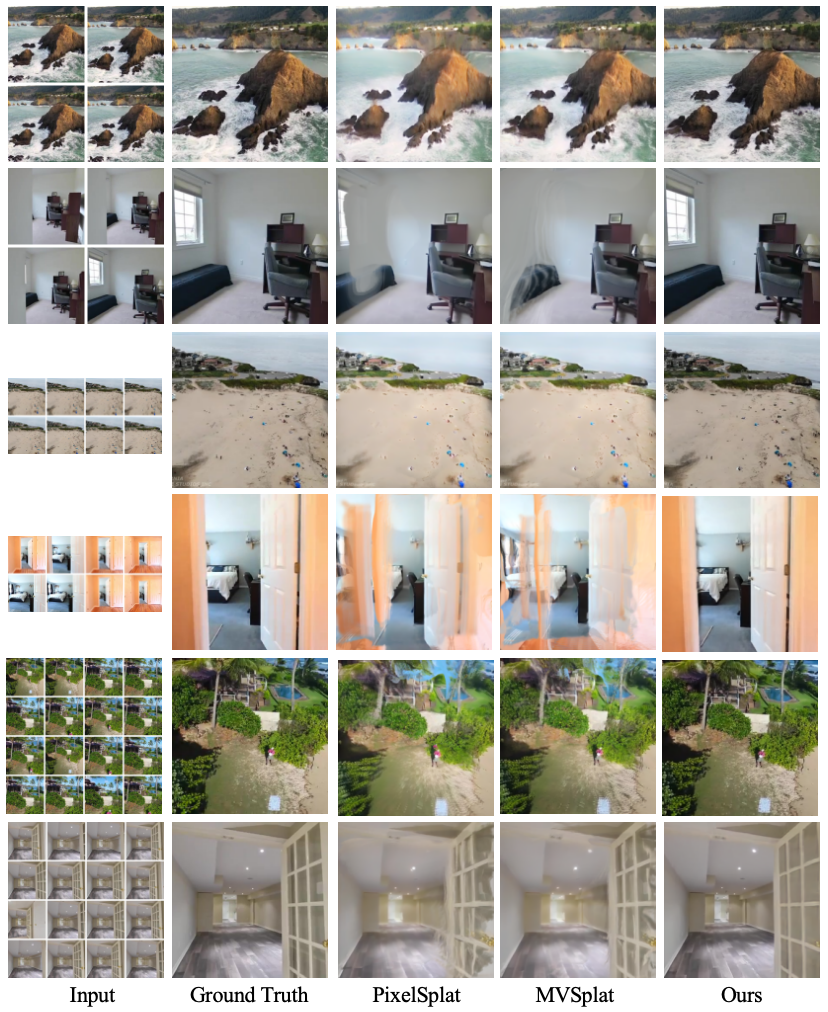
\includegraphics[width=\textwidth]{fig/main_result.png}
    \caption{Visualization results on RealEstate10K~\cite{RealEstate10K2018} and ACID~\cite{ACID2021ICCV} benchmarks. We evaluate all models with 4, 8, 16 views as input and subsequently test on three target novel views.}
    \label{fig: main result visual} 
    \vspace{-0.5cm}
\end{figure}

\subsection{Multi-view Scene Reconstruction and Synthesis}~\label{sec:main exp}
\textbf{Datasets.} We conduct experiments on two large-scale datasets, including RealEstate10K~\cite{RealEstate10K2018} and ACID~\cite{ACID2021ICCV}. RealEstate10K dataset comprises video frames of real estate scenes, which are split into 67,477 scenes for training and 7,289 scenes for testing.
ACID dataset consists of natural landscape scenes, with 11,075 training scenes and 1,972 testing scenes. 
For two-view inputs, our model is trained with two views as input, and subsequently tested on three target novel views for each scene. For multi-view inputs, we construct challenging subsets for RealEstate10K and ACID across a broader range of each scenario to evaluate model performance. We select 4, 8 and 16 views as reference views, and evaluate pixelSplat~\cite{pixelSplat2023arXiv}, MVSplat~\cite{MVSplat2024arXiv} and ours on the same target novel views.

\textbf{Implementation details.} Our model is trained with two input views for each scene on a single A6000 GPU, utilizing the Adam optimizer. Following the instruction of previous methods~\cite{pixelSplat2023arXiv, MVSplat2024arXiv}, all experiments are conducted on $256\times256$ resolutions for fair comparison. The image backbone is initialized by the feature extractor and cost volume representations in MVSplat~\cite{MVSplat2024arXiv}. The number of graph layer is set to 2. The training loss is a linear combination of MSE and LPIPS~\cite{LPIPS2018CVPR} losses, with loss weights of 1 and 0.05.

\textbf{Results.} As shown in Table~\ref{tab:multi view results re10k} and Table~\ref{tab:multi view results acid}, our Gaussian Graph benefits from increasing input views, whereas both pixelSplat~\cite{pixelSplat2023arXiv} and MVSplat~\cite{MVSplat2024arXiv} exhibit declines in performance. This distinction highlights the superior efficiency of our approach, which achieves more effective 3D representation with significantly fewer Gaussians compared to pixel-wise methodologies. For 4 view inputs, our method outperforms MVSplat~\cite{MVSplat2024arXiv} by about 4dB on PSNR with more than $2\times$ fewer Gaussians. For more input views, the number of Gaussians in previous methods increases linearly, while our GGN only requires a small increase.
Considering that previous methods suffer from the redundancy of Gaussians, we adopt these models with multi-view inputs and preserve Gaussians from two input views for rendering.
Under this circumstance, pixelSplat~\cite{pixelSplat2023arXiv} and MVSplat~\cite{MVSplat2024arXiv} achieve better performance than before, because the redundancy of Gaussians is alleviated to some degree. However, the lack of interaction at Gaussian level limits the quality of previous methods.
In contrast, our Gaussian Graph can significantly enhance performance by leveraging additional information from extra views. Visualization results in Figure~\ref{fig: main result visual} also indicate that pixelSplat~\cite{pixelSplat2023arXiv} and MVSplat~\cite{MVSplat2024arXiv} tend to suffer from artifacts due to duplicated and unnecessary Gaussians in local areas, which increasingly affects image quality as more input views are added.

% inference efficiency
\begin{table}[t]
    \centering
    \caption{Inference time comparison across different views. We train our model on 2 input views and report the inference time for 4 views, 8 views, and 16 views, respectively.}
    \vspace{0.2cm}
    \setlength{\tabcolsep}{4mm}{\begin{tabular}{ccccccc}
        \toprule
        \cmidrule(lr){3-6}
        & & 2 views & 4 views & 8 views & 16 views \\
        \cmidrule(lr){1-6}
        pixelSplat~\cite{pixelSplat2023arXiv} & 125.4 & 137.3 & 298.8 & 846.5 & 2938.9 \\
        MVSplat~\cite{MVSplat2024arXiv} & 12.0 & 60.6 & 126.4 & 363.2 & 1239.8 \\
        Ours & 12.5 & 75.6 & 148.1 & 388.8 & 1267.5 \\
        \bottomrule
    \end{tabular}}
    \label{tab:inference time result}
\end{table}

\begin{figure}[t]
    \centering
    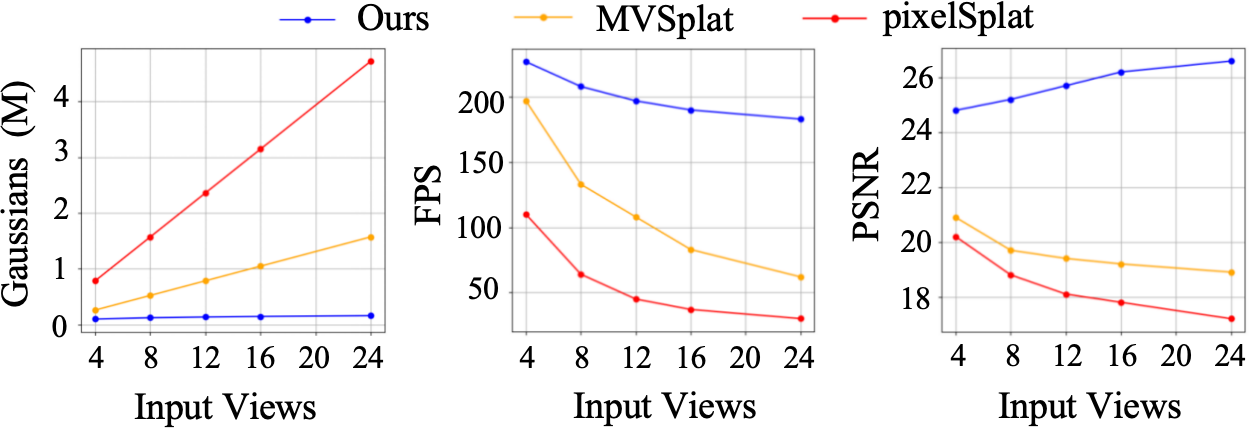
\includegraphics[width=0.8\textwidth]{fig/efficiency.png}
    \caption{Efficiency analysis. We report the number of Gaussians (M), rendering frames per second (FPS) and reconstruction PSNR of pixelSplat~\cite{pixelSplat2023arXiv}, MVSplat~\cite{MVSplat2024arXiv} and our GGN.}
    \label{fig: efficiency} 
    \vspace{-0.4cm}
\end{figure}

% cross-dataset visualization
\begin{figure}[h]
    \centering
    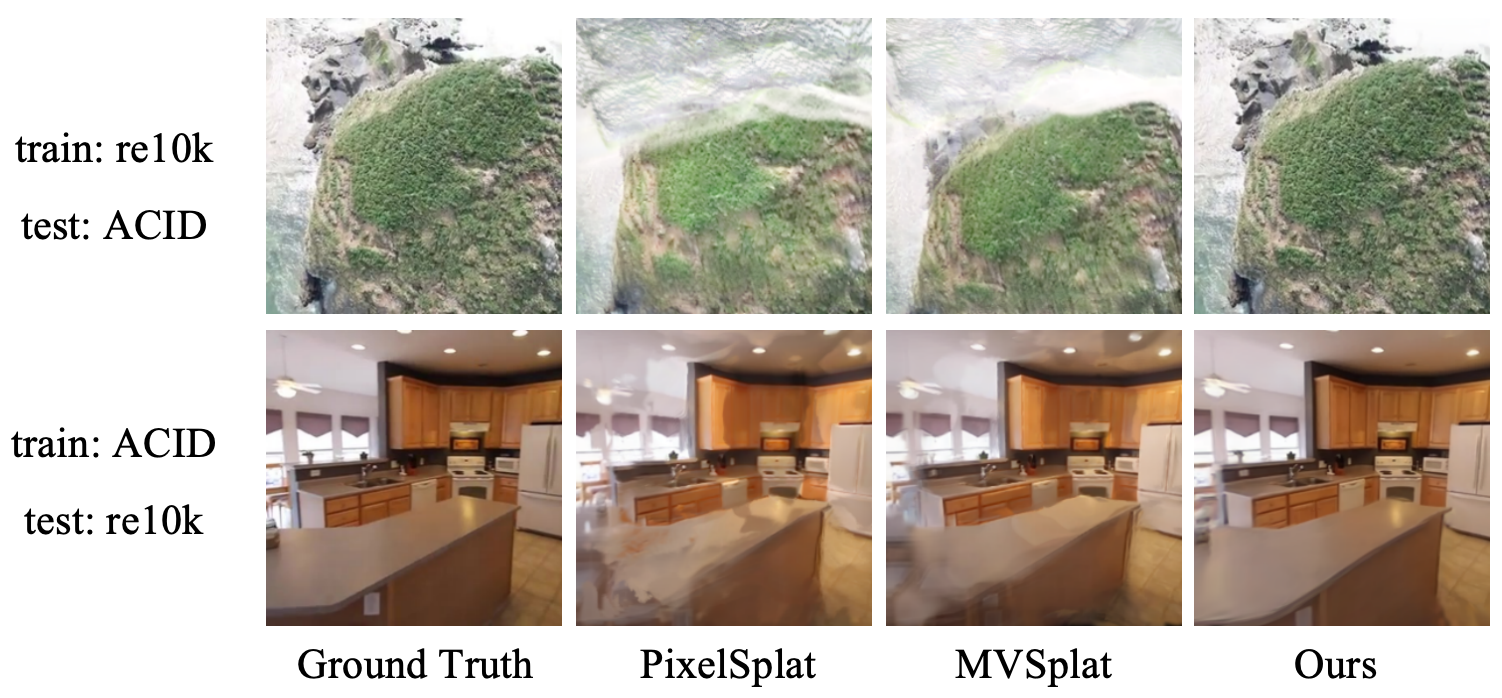
\includegraphics[width=0.9\textwidth]{fig/cross_dataset_visual.png}
    \caption{Visualization of model performance for cross-dataset generalization on RealEstate10K~\cite{RealEstate10K2018} and ACID~\cite{ACID2021ICCV} benchmarks.}
    \label{fig: cross-dataset visual} 
    \vspace{-0.3cm}
\end{figure}

\subsection{Efficiency Analysis.}~\label{sec:efficiency exp}
% efficiency
In addition to delivering superior rendering quality, our Gaussian Graph network also enhances efficiency in 3D representations. As illustrated in Figure~\ref{fig: efficiency}, when using 24 input images, our model outperforms MVSplat by 8.6dB on PSNR with approximately one-tenth the number of 3D Gaussians and more than three times faster rendering speed. Additionally, we compare the average inference time of our model with pixel-wise methods in Table~\ref{tab:inference time result}. Our GGN is able to efficiently remove duplicated Gaussians and enhance Gaussian-level interactions, which allows it to achieve superior reconstruction performance with comparable inference speed to MVSplat. 






\begin{table}[t]
    \centering
    \caption{Cross-dataset performance and efficiency comparisons on RealEstate10K~\cite{RealEstate10K2018} and ACID~\cite{ACID2021ICCV} benchmarks. We assign eight views as reference and test on three target views for each scene.}
    \vspace{0.2cm}
    \begin{tabular}{cc|cccccc}
        \toprule
        Train Data& Test Data & Method & PSNR↑ & SSIM↑ & LPIPS↓ & Gaussians (K)& FPS \\
        \midrule
        \multirow{3}{*}{ACID}& \multirow{3}{*}{re10k}& pixelSplat & 18.65 & 0.715 & 0.276 & 1572 & 64 \\
        & & MVSplat & 19.17 & 0.731 & 0.270 & 524 & 133 \\
        & & Ours & 24.75 & 0.759 & 0.252 & 126 & 208 \\
        \cmidrule{1-8}
        \multirow{3}{*}{re10k}& \multirow{3}{*}{ACID}& pixelSplat & 19.75 & 0.724 & 0.264 & 1572 & 64 \\
        & & MVSplat & 20.58 & 0.735 & 0.239 & 524 & 133 \\
        & & Ours & 25.21 & 0.762 & 0.234 & 126 & 208 \\
        \bottomrule
    \end{tabular}
    \label{tab:cross_dataset}
    \vspace{-0.4cm}
\end{table}

% Ablation Table
\begin{table}[t]
\centering
\caption{Ablation study results of GGN on RealEstate10K~\cite{RealEstate10K2018} benchmarks. Each scene takes eight reference views and renders three novel views.}
\vspace{0.2cm}
\begin{tabular}{lcccc}
    \toprule
    Models & PSNR↑ & SSIM↑ & LPIPS↓ & Gaussians (K) \\
    \midrule
    Gaussian Graph Network & 25.15 & 0.786 & 0.232 & 126 \\
    w/o Gaussian Graph linear layer & 24.72 & 0.778 & 0.246 & 126 \\
    w/o Gaussian Graph pooling layer & 20.25 & 0.725 & 0.272 & 524 \\
    Vanilla & 19.74 & 0.721 & 0.279 & 524 \\
    \bottomrule
    \vspace{-0.6cm}
\end{tabular}
\label{tab:ablation study}
\end{table}

\subsection{Cross Dataset Generalization.}~\label{sec:cross-dataset exp}
% Our Gaussian Graph Network is designed to effectively encode multi-view correlations and universal 3D geometry features into a limited number of 3D Gaussians, which remains invarient and robust across various 3D scenarios. 
To further demonstrate the generalization of Gaussian Graph Network, we conduct cross-dataset experiments. Specifically, all models are trained on RealEstate10K~\cite{RealEstate10K2018} or ACID~\cite{ACID2021ICCV} datasets, and are tested on the other dataset without any fine-tuning. Our method constructs the Gaussian Graph according to the relations of input views. As shown in Table~\ref{tab:cross_dataset}, our GGN consistently outperforms pixelSplat~\cite{pixelSplat2023arXiv} and MVSplat~\cite{MVSplat2024arXiv} on both benchmarks. 



\subsection{Ablations}~\label{sec:ablation exp}
To investigate the architecture design of our Gaussian Graph Network, we conduct ablation studies on RealEstate10K~\cite{RealEstate10K2018} benchmark. We first introduce a vanilla model without Gaussian Graph Network. Then, we simply adopt Gaussian Graph linear layer to model relations of Gaussian groups from multiple views. Furthermore, we simply introduce Gaussian Graph pooling layer to aggregate Gaussian groups to obtain efficient representations. Finally, we add the full Gaussian Graph Network model to both remove duplicated Gaussians and enhance Gaussian-level interactions.

\textbf{Gaussian Graph linear layer.} The Gaussian Graph linear layer serves as a pivotal feature fusion block, enabling Gaussian Graph nodes to learn from their neighbor nodes. The absence of linear layers leads to a performance drop of 0.43 dB on PSNR.
% As illustrated in Table ~\ref{tab:ablation study}, the encoding of multi-view geometry alignment and correlations provides significant guidance for rendering novel views.


\textbf{Gaussian Graph pooling layer.} The Gaussian Graph pooling layer is important to avoid duplicate and unnecessary Gaussians, which is essential for preventing artifacts and floaters in reconstructions and speeding up the view rendering process. As shown in Table~\ref{tab:ablation study}, the introduction of Gaussian Graph pooling layer improves the rendering quality by 4.9dB on PSNR and reduces the number of Gaussians to nearly one-fourth. 
    